\documentclass[a4paper,11pt] {article}
\usepackage[spanish]{babel}
\usepackage[utf8]{inputenc}
\usepackage{caratula}
\usepackage{a4wide}
\usepackage{graphicx}
% \usepackage{dot2texi}
% \usepackage{graphs}

\begin{document}

\titulo{Trabajo Pr\'actico}
\fecha{10/12/2009}
\materia{Sistemas Operativos}
\grupo{Grupo Nro. 10}
\integrante{Dinota, Mat\'ias}{076/07}{matiasgd@gmail.com}
\integrante{Leveroni, Luciano}{360/07}{lucianolev@gmail.com}
\integrante{Mosteiro, Agust\'in}{125/07}{agustinmosteiro@gmail.com}

\maketitle

\bigskip
\section*{Aclaraciones generales}

Antes de comenzar el an\'alisis de cada ejercicio, cabe mencionar lo siguiente: 

\begin{itemize}
 \item En los ejercicios donde se pida realizar un script o un módulo del kernel, se mostrará el código fuente en cuestión que realiza lo pedido junto con comentarios explicativos de su funcionamiento dentro del mismo. Posteriormente, se hará un breve resumen de la funcionalidad del mismo pero sin mencionar detalles implementativos (ya que se encuentran en los comentarios).
\end{itemize}

\section{Comandos b\'asicos de Unix}

\begin{enumerate}
	\item \textbf{pwd}: El comando \textit{pwd} se utiliza para imprimir en pantalla el directorio actual de trabajo. De esta manera, ejecutando primero los comandos pedidos y luego el comando \textit{pwd} se obtuvo lo siguiente:
	\begin{enumerate}
		\item \textbf{cd /usr/bin}.El directorio actual pasa a ser \textbf{/usr/bin}.
		\item \textbf{cd}.El directorio actual pasa a ser \textbf{/home/tpsisop}.
		\item Al no ingresar ning\'un par\'ametro, el comando \textit{cd} cambia el directorio actual al directorio personal del usuario actual.
	\end{enumerate}
	\item \textbf{cat}: El comando \textit{cat} es utilizado para imprmir en pantalla el contenido de un archivo. Podemos ver entonces el contenido del archivo \textbf{/home/tpsisop/.profile} con el comando \textbf{cat /home/tpsisop/.profile}.
	El contenido del archivo es:
	\begin{verbatim}
# ~/.profile: executed by the command interpreter for login shells.
# This file is not read by bash(1), if ~/.bash_profile or ~/.bash_login
# exists.
# see /usr/share/doc/bash/examples/startup-files for examples.
# the files are located in the bash-doc package.

# the default umask is set in /etc/profile
#umask 022

# if running bash
if [ -n "$BASH_VERSION" ]; then
    # include .bashrc if it exists
    if [ -f "$HOME/.bashrc" ]; then
       . "$HOME/.bashrc"
    fi
fi

# set PATH so it includes user's private bin if it exists
if [ -d "$HOME/bin" ] ; then
    PATH="$HOME/bin:$PATH"
fi
	\end{verbatim}
	\item \textbf{find}: Este comando es utilizado para buscar archivos dentro de un determinado directorio. Como se pide buscar archivos que comienzan con \textit{vmlinuz} en todo el sistema el comando que se ejecut\'o fue \textbf{find / vmlinuz*} (el directorio ra\'iz se especifica con /). El \'unico archivo encontrado es \textbf{/vmlinuz}.
	\item \textbf{mkdir}: El comando \textit{mkdir} se utiliza para generar nuevos directorios. De esta manera, se gener\'o el directorio especificado utilizando el comando \textbf{mkdir /home/tpsisop/tp}.
	\item \textbf{cp}: El comando \textit{cp} es utilizado para copiar archivos entre distintos directorios. Se copi\'o entonces el archivo \textit{/etc/passwd} utilizando el comando \textbf{cp /etc/passwd /home/tpsisop/tp/}.
	\item \textbf{chgrp}: El comando \textit{chgrp} permite cambiar el grupo de un archivo. Se cambi\'o el grupo del archivo \textit{/home/tpsisop/tp/passwd} a nuestro grupo utilizando el comando \textbf{chgrp tpsisop /home/tpsisop/tp/passwd}.
	\item \textbf{chown}: El comando \textit{chown} permite cambiar el dueño de un archivo. Se cambi\'o el dueño del archivo \textit{/home/tpsisop/tp/passwd} a nuestro usuario utilizando el comando \textbf{chown tpsisop /home/tpsisop/tp/passwd}.
	\item \textbf{chmod}: El comando \textit{chmod} permite cambiar los permisos de acceso a un archivo. De esta manera, se cambiaron los permisos del archivo \textit{/home/tpsisop/tp/passwd}.
		\begin{itemize}
			\item Para que el propietario tenga permisos de lectura, escritura y ejecuci\'on: \textbf{chmod u$+$rwx /home/tpsisop/tp/passwd}.
			\item Para que el grupo tenga s\'olo permisos de lectura y ejecuci\'on: \textbf{chmod g$-$w$+$rx /home/tpsisop/tp/passwd}.
			\item Para que el resto tenga s\'olo permisos de ejecuci\'on: \\ \textbf{chmod o$-$rw$+$x /home/tpsisop/tp/passwd}.
		\end{itemize}
	\item \textbf{grep}: El comando \textit{grep} toma una expresión regular de la línea de comandos, lee la entrada est\'andar o una lista de archivos, e imprime las l\'ineas que contengan coincidencias para la expresi\'on regular. Para mostrar las l\'ineas de \textit{/etc/hosts} que contienen el texto ``localhost'' se utiliz\'o el comando \textbf{grep localhost /etc/hosts} arrojando el siguiente resultado:
		\begin{verbatim}
	 			127.0.0.1	localhost
			::1     ip6-localhost ip6-loopback
		\end{verbatim}
Luego para mostrar las l\'ineas de todos los archivos en \textit{/etc} que contienen el texto ``POSIX'' se utiliz\'o el comando \textbf{grep -r POSIX | grep -v} en la carpeta \textit{/etc}.
	\item \textbf{passwd}: El comando \textit{passwd} se utiliza para cambiar la contraseña de un usuario. Cambiamos entonces la password de nuestro usuario a \textit{guiguigui} con el comando \textbf{passwd}.
	\item \textbf{rm}: El comando \textit{rm} se utiliza para remover archivos. Se borr\'o el archivo \\ \textit{/home/tpsisop/tp/passwd} con el comando \textbf{rm /home/tpsisop/tp/passwd}.
	\item \textbf{ln}: El comando \textit{ln} es utilizado para enlazar archivos. Se enlazaron los archivos con los comandos \textbf{ln /etc/passwd /tmp/contra1}, \textbf{ln /etc/passwd /tmp/contra2} y \textbf{ln -s /etc/passwd /tmp/contra3} respectivamente.
	\item \textbf{mount}: El comando \textit{mount} se utiliza para montar dispositivos y particiones para su uso por el sistema operativo. Se mont\'o el CD-ROM de instalacion de Ubuntu JeOS con el comando \textbf{mount /dev/sr0/ /home/tpsisop/tp/}. El contenido del directorio es:
	\begin{verbatim}
		-r-xr-xr-x 1 root root   942 2008-04-22 03:07 cdromupgrade
		dr-xr-xr-x 3 root root  2048 2009-07-14 13:23 dists
		dr-xr-xr-x 3 root root  2048 2009-07-14 13:23 doc
		dr-xr-xr-x 3 root root  2048 2009-07-14 13:24 install
		dr-xr-xr-x 2 root root 12288 2009-07-14 13:24 isolinux
		-r--r--r-- 1 root root 47110 2009-07-14 13:24 md5sum.txt
		dr-xr-xr-x 2 root root  2048 2009-07-14 13:23 pics
		dr-xr-xr-x 4 root root  2048 2009-07-14 13:23 pool
		dr-xr-xr-x 2 root root  2048 2009-07-14 13:23 preseed
		-r--r--r-- 1 root root   228 2009-07-14 13:23 README.diskdefines
		lr-xr-xr-x 1 root root     1 2009-07-14 13:23 ubuntu -> .
	\end{verbatim}
	Se utiliz\'o el comando \textbf{mount} para mostrar los siguientes \textit{filesystems} montados:
	\begin{verbatim}
		/dev/sda1 on / type ext3 (rw,relatime,errors=remount-ro)
		proc on /proc type proc (rw,noexec,nosuid,nodev)
		/sys on /sys type sysfs (rw,noexec,nosuid,nodev)
		varrun on /var/run type tmpfs (rw,noexec,nosuid,nodev,mode=0755)
		varlock on /var/lock type tmpfs (rw,noexec,nosuid,nodev,mode=1777)
		udev on /dev type tmpfs (rw,mode=0755)
		devshm on /dev/shm type tmpfs (rw)
		devpts on /dev/pts type devpts (rw,gid=5,mode=620)
		/dev/scd0 on /home/tpsisop/tp type iso9660 (ro)
	\end{verbatim}
	\item \textbf{df}: Se utiliz\'o el comando \textit{df} para mostrar el espacio libre de los \textit{filesystems} montados:
	\begin{verbatim}
		Filesystem            Size  Used Avail Use% Mounted on
		/dev/sda1             494M  423M   46M  91% /
		varrun                252M   32K  252M   1% /var/run
		varlock               252M     0  252M   0% /var/lock
		udev                  252M   40K  252M   1% /dev
		devshm                252M     0  252M   0% /dev/shm
		/dev/scd0             101M  101M     0 100% /home/tpsisop/tp
	\end{verbatim}
	\item \textbf{ps}: El comando \textit{ps} imprime informaci\'on relativa a los procesos en ejecuci\'on.
	\item \textbf{unmount}: Se desmont\'o el CD-ROM de instalaci\'on de Ubuntu JeOS con el comando \textbf{unmount /dev/scd0}.
	\item \textbf{uptime}: La maquina virtual lleva 58 minutos de ejecuci\'on. Esto se corrobor\'o con el comando \textbf{uptime}.
	\item \textbf{uname}: La versi\'on de kernel utilizada es la 2.6.24-24-virtual. Esta informaci\'on se obtuvo utilizando el comando \textbf{uname -a}.

\end{enumerate}

\section{Comandos Extendidos de Unix}

\begin{enumerate}
	\item Para escribir HOLA en la pantalla cada vez que se loguee un usuario se agreg\'o la siguiente l\'inea al archivo 	/etc/bash.bashrc:	\textbf{echo ``HOLA''}. Esto funciona debido a que el programa \textit{bash} se corre una vez que un 	usuario se loguea. De esta manera al agregar la l\'inea mencionada en la configuraci\'on de arranque del programa se 	logr\'o el objetivo requerido.
	
	Para escribir BUENOS DIAS en la pantalla cada vez que se encienda la m\'aquina se agreg\'o la siguiente l\'inea al 	archivo \textit{/etc/rc.local}: \textbf{echo ``BUENOS DIAS''}. Como \textit{local} es el \'ultimo script que se ejecuta 	luego	del booteo de la m\'aquina, al agregar la l\'inea mencionada en la configuraci\'on de dicho scritp podremos 	leer el mensaje en pantalla previo al proceso de logueo.
	
	Para escribir ADIOS en la pantalla cada vez que se desloguee un usuario se cre\'o un archivo llamado \textit{logout} en el directorio /etc. El contenido del archivo es el siguiente: \textbf{echo ``ADIOS''}. Luego, se agreg\'o en el 	archivo \textit{/etc/rc.local} la siguiente l\'inea: \textbf{trap '/etc/logout;exit' 0}. Cuando un usuario se 	desloguea, el script \textit{local} se cierra. De esta manera, al agregar el \textit{trap} logramos que antes de 	cerrarse llame al archivo \textit{logout} para que cumpla con lo pedido.
	
	Para escribir HASTA LA VISTA BABY en la pantalla cada vez que se apague la m\'aquina se agreg\'o la siguiente l\'inea 	al archivo \textit{/etc/rc0.d}: \textbf{echo ``HASTA LA VISTA BABY''}. El archivo mencionado corresponde al \textit{run 	level 0} que corresponde al apagado de la m\'aquina. Al agregar el comando para imprimir en su configuraci\'on 	logramos que imprima el mensaje antes de apagarse.
	
	\item Para montar una imagen de floppy se utiliz\'o el siguiente comando:
		\textbf{mount -o loop imagen.img /media/floppy1/}
		
		Para montar una imagen iso se utiliz\'o el siguiente comando:
		\textbf{mount -o loop imagen.iso /media/iso/}
		
	\item Se agreg\'o un alias en el archivo .bashrc sin modificar su fecha (timestamp). Para esto se utiliz\'o el comando \textbf{touch -t timestamp}. El timestamp del archivo previo a la modificaci\'on se obtuvo con el comando  \textbf{ls -l}.
	El d\'ia y la hora del sistema se modific\'o con el comando \textbf{date timestamp}.
	
	\item Con el comando \textit{last} podemos ver los ultimos usuarios que se han logueado en el sistema y que 	terminales usaron, asi como tambi\'en los \'ultimos reinicios del sistema. Entre la informaci\'on que nos muestra se 	encuentran de izquierda a derecha, el usuario, la terminal que uso, el kernel con que arranc\'o este usuario, la 	fecha del login, la hora de acceso y la hora de salida, asi como un resumen (entre par\'entesis) de la cantidad de 	horas que este usuario estuvo en el sistema.
	\item \textbf{STDOUOT}
		\begin{enumerate}
			\item Se guard\'o la informaci\'on en el archivo \textit{config} utilizando el comando \textbf{ls -R /etc 			$>$ /home/tpsisop/tp/config}. Con el comando $>$ se logra que la salida del primer par\'ametro se escriba 			en el archivo especificado.
			\item El archivo \textit{config} posee 789 l\'ineas, 5061 palabras y 39070 caracteres. Se obtuvo la 				informaci\'on mediante el comando \textbf{wc config}.
			\item Se agrego el contenido ordenado del archivo \textit{/etc/passwd} al final del archivo \textit				{config} con el comando \textbf{sort /etc/passwd $>>$ /home/tpsisop/tp/config}. Con \textit{sort} 				ordenamos el contenido del primer archivo y con $>>$ agregamos la informaci\'on al final del segundo par\'ametro.
			\item El archivo \textit{config} posee 813 l\'ineas, 5090 palabras y 40051 caracteres. Se obtuvo la 				informaci\'on mediante el comando \textbf{wc config}.
		\end{enumerate}
	\item \textbf{Pipes}: Se realiz\'o lo pedido ejecutando el siguiente comando: \textbf{ls -l /usr/bin/a* | grep apt | 	wc}. Con el argumento -l logramos que \textit{ls} presente los archivos de manera listada. Al especificar la ruta 	\textit{/usr/bin/a*} logramos que se muestren solo los archivos que comienzan con la letra a. Luego con el primer 	pipe le pasamos este resultado al comando \textit{grep} para que solo muestre las l\'ineas de dichos archivos que 	contengan el texto apt. Finalmente con el segundo pipe mostramos en pantalla la informaci\'on requerida mediante el 	comando \textit{wc}.
\end{enumerate}

\section*{Scripting}

\begin{enumerate}
	\item Para realizar lo pedido, se hizo uso del demonio \textbf{cron}, muy popular en los sistemas Linux, que permite realizar tareas en forma programada. Mediante el comando \textbf{sudo crontab -e} se agregó la siguiente información al archivo correspondiente a las tareas programadas del usuario \textit{root}:

	\begin{verbatim}
	# m h dom mon dow command
	*/5 * * * * echo "HOLA" > /dev/console
	22 15 * * * echo "HOLA" > /dev/console
	\end{verbatim}

	La primer línea indica que se debe mostrar en la consola el mensaje ``HOLA'' cada 5 minutos. Asimismo, la segunda línea será la encargada de que el mensaje se muestre a las 22:15 (hora elegida arbitrariamente). 

	Para terminar, cabe hacer la siguiente aclaración: El demonio no suele ser utilizado para mostrar información en pantalla, sino que por defecto envía por mail las salidas de los comandos/scripts a ejecutarse. Por esta razón, fue necesario enviar la salida al dispositivo \textit{/dev/console}. Por este mismo motivo, fue necesario que estas tareas programadas estén asociadas al usuario \textit{root} ya que solo él tiene acceso de escritura por defecto a este dispositivo.

	\item Para poder realizar las tareas de control de usuario pedidas, se optó por utilizar el lenguaje \textbf{awk} debido a que permite fácilmente el procesamiento de archivos. A continuación, el \textit{script} programado en cuestión:

	\begin{verbatim}
#!/usr/bin/awk -f

BEGIN { 
    print "-> Procesando lista de usuarios..."
    pwdfile = "/etc/passwd"
    #El separador de fields es : en pwdfile
    FS = ":"
    #Guardo en un array 'users' los usuarios de passwd 
    #indexados por el userid
    while( (getline < pwdfile) > 0 ) {
        userid = $3
        login = $1
        users[userid] = login
    }
    close(pwdfile)
    #Seteo el separador de fields en espacio para 
    #la lectura del archivo de entrada
    FS = " "
}
{
    useridF = $1
    #Si el id existia en el pwdfile
    #entonces debo editar la info de ese id, sino agregarlo
    if( users[useridF] ) {
        #El login es el obtenido de /etc/passwd que se corresponde
        #con el userid del archivo de entrada
        login = users[useridF]

        #Puede ser U o G, U cambiar login, G cambiar grupo
        tipoCambioF = $2
        if( tipoCambioF == "U" ) {
            loginF = $3
            paramsCommand = "-l " loginF
        } else if( tipoCambioF == "G" ) {
            grupoF = $3
            paramsCommand = "-g " grupoF
        }

        #Si hay 4 parametros es porque tambien hay que cambiar clave
        if( NF == 4) { 
            claveF = $4
            encClave = "`perl -e \"print crypt('" claveF "', 'Q9')\"`"
            paramsCommand = paramsCommand " -p " encClave
        }

        print "Modificando informacion del usuario con id " useridF "..."
        thecommand = "usermod " paramsCommand " " login
        system(thecommand)
    } else {
        #El login es el especificado en el archivo de entrada
        login = $3

        #Si hay 4 parametros es que no pasaron el grupo,
        #si hay 5 es porque hay q asignar grupo
        if( NF == 4 ) { 
            claveF = $4
            paramsCommand = ""
        } else if ( NF == 5 ) {
            grupoF = $4
            claveF = $5
            paramsCommand = "-g " grupoF
        }

        encClave = "`perl -e \"print crypt('" claveF "', 'Q9')\"`"
        paramsCommand = paramsCommand " -p " encClave " -u " useridF

        print "Agregando al usuario con id " useridF "..."
        thecommand = "useradd " paramsCommand " " login
        system(thecommand)
    }
}
END {
    print "-> Se han realizado las modificaciones en el sistema"
}
	\end{verbatim}

	Como se puede observar, el script primero procesa el archivo /etc/passwd para obtener información de los usuarios actuales del sistema. Luego, procesa el archivo de entrada (la lista con el formato indicado en el ejercicio) y se va construyendo el comando adecuado a ejecutar. En caso de que se vaya a modificar la información de un usuario, se utilizará el comando \textbf{usermod}, mientras que para agregar uno nuevo el comando es \textbf{useradd}. Para encriptar las claves, se usó la función \textit{crypt()} a través del intérprete de \textbf{perl}.

\end{enumerate}

\section*{Ejecuci\'on de procesos en background}

El programa en lenguaje C que se pide crear se trata b\'asicamente de un ciclo infinito que imprime distintos n\'umeros en pantalla. El ejecutable correspondiente se obtuvo mediante el comando \textbf{gcc}. 

El primer paso fue correr el proceso en \textit{foreground}. Para esto simplemente se lo ejecut\'o con el comando \textbf{./loop}. Cuando se corre un proceso en \textit{foreground} el usuario debe esperar que este termine antes de poder ejecutar otro. En este caso entonces el proceso imprime indefinidamente n\'umeros en pantalla sin que podamos volver a tener el control de la consola. Para solucionar esto matamos el proceso con las teclas Ctrl+c.

El segundo paso consisti\'o en ejecutar el proceso en \textit{background}. Esto se logro ejecutando el comando \textbf{./loop $>$ /dev/null \&}. Con $>$ evitamos que imprima en pantalla enviando los datos a \textit{/dev/null} y con \& indicamos que el proceso debe correrse en \textit{background}. A diferencia de los procesos que corren en \textit{foreground}, la consola no debe esperar que los procesos terminen para poder correr otros. De esta manera, luego de ejecutar el comando mencionado tenemos el control de la consola nuevamente. Para terminar procesos que se encuentren corriendo en \textit{background} se utiliza el comando \textit{kill} seguido del ID del proceso. Los IDs de los distintos procesos que se encuentran corriendo en el sistema se pueden obtener mediante el comando \textit{top}.

\section*{IPC y sincronizaci\'on}

\begin{enumerate}

	\item \textbf{Pipes}

	Para lograr exclusi\'on mutua entre dos procesos utilizando un solo pipe utilizamos la idea vista en las diapositivas de pipes de las clases de TP. El c\'odigo del programa es el siguiente:
	\begin{verbatim}
#include <stdio.h>
#include <stdlib.h>
#include <sys/wait.h>

int main()
{
        int pfd[2];
        pid_t cpid;
        char buf[80];

        if(pipe(pfd)== -1) {
            perror("pipe");
            exit(EXIT_FAILURE);
        }


        cpid = fork();
        if (cpid == -1){
            perror("fork");
            exit(EXIT_FAILURE);
        }


        if (cpid == 0){
            close(pfd[1]);
            printf("Se ejecuta el hijo\n");
            read(pfd[0], &buf, 1);
            close(pfd[0]);
            exit(EXIT_SUCCESS);

        }else {
            close(pfd[0]);
            printf("Se ejecuta el padre\n");
            write(pfd[1], &buf, 1);
            close(pfd[1]);
            wait(NULL);
            exit(EXIT_SUCCESS);
        }

}
	\end{verbatim}

	Se puede apreciar como inicialmente se crea un pipe y se chequea que no haya ning\'un error. A continuaci\'on, con el comando \textit{fork}, se genera un proceso hijo que ser\'a id\'entico al padre salvo por su PID y se chequea nuevamente que no haya habido errores. De esta manera, a trav\'es de la variable \textit{cpid} logramos establecer si el permiso de ejecuci\'on lo tendra hijo o padre y utilizando el pipe creado podremos realizar la exclusi\'on mutua entre ambos procesos permitiendo al hijo leer del pipe sin ejecuci\'on del padre y a este \'ultimo escribir sin que el hijo se este ejecutando.

	\item \textbf{Threads}

	\begin{verbatim}
	#include <stdio.h>
	#include <stdlib.h>
	#include <pthread.h>
	
	#define BSIZE 10
	
	typedef struct {
	  char         buf[BSIZE];
	  pthread_mutex_t        lock;
	  pthread_cond_t        less;
	  pthread_cond_t        more;
	  int         nextin;
	  int         nextout;
	  int         occupied;
	} buffer_t;
	
	void consumer(buffer_t * b);
	void producer(buffer_t * b);
	char consume(buffer_t * b);
	void produce(buffer_t * b, char item);
	
	int main(int argc, char* argv[]) {
	  pthread_t threads[2];
	  buffer_t buffer;
	  pthread_mutexattr_t mutex_attr;
	  pthread_condattr_t cond_attr;
	  buffer.occupied = 0;
	  buffer.nextin = 0;
	  buffer.nextout = 0;

	  int i;
	  for(i = 0; i < BSIZE; i++) {
	    buffer.buf[i] = 0;
	  }
	
	  pthread_mutexattr_init(&mutex_attr);
	  pthread_mutexattr_setpshared(&mutex_attr,PTHREAD_PROCESS_SHARED);
	  pthread_mutex_init(&buffer.lock, &mutex_attr);
	  pthread_condattr_init(&cond_attr);
	  pthread_condattr_setpshared(&cond_attr, PTHREAD_PROCESS_SHARED);
	  pthread_cond_init(&buffer.less, &cond_attr);
	  pthread_cond_init(&buffer.more, &cond_attr);

	  int rc;
	  rc =  pthread_create(&threads[0], NULL, producer, (void*)&buffer);
	  if (rc) {
	    printf("Error al crear el thread 0");
	    exit(1);
	  }

	  rc =  pthread_create(&threads[1], NULL, consumer, (void*)&buffer);
	  if (rc) {
	    printf("Error al crear el thread 1");
	    exit(1);
	  }
	  pthread_exit(0);
	}
	
	void consumer(buffer_t * b){
	  char item;
// 	  printf("Consumidor - %d\n", getpid());
	  FILE* salida = fopen("salida.txt","w");
	  while (1) { 
	    if(salida == NULL) {
	      exit(0);
	    }
	    item = consume(b);
	    if (item == '\0')
	      break;
	    fputc((int)item,salida);
	  }
	  fclose(salida);
	}
	
	void producer(buffer_t * b) {
	  char item[20];
	  //printf("Productor - %d\n", getpid());
	  while (1) {
	    printf("Introduzca item: ");
	    scanf("%s", item);
	
	    if (item[0] == 'q') {
	      produce(b, '\0');
	      break;
	    } else
	      produce(b, (char) item[0]);
	    }
	}
	
	char consume(buffer_t * b){
	  char         item;
	  pthread_mutex_lock(&b->lock);
	
	  while (b->occupied == 0)
	    pthread_cond_wait(&b->more, &b->lock);

	  printf("Consume\n");
	  item = b->buf[b->nextout];

	  if(b->nextout != 0)
	    b->nextout--;

	  b->nextin--;
	  b->occupied--;
	
	  pthread_cond_signal(&b->less);
	  pthread_mutex_unlock(&b->lock);
	  return (item);
	}
	
	void produce(buffer_t * b, char item) {
	  pthread_mutex_lock(&b->lock);
	
	  while (b->occupied == BSIZE)
	    pthread_cond_wait(&b->less, &b->lock);

	  printf("Produce\n");
	  b->buf[b->nextin] = item;
	
	  b->nextin++;
	  if(b->nextin > 1)
	    b->nextout++;

	  b->occupied++;
	  pthread_cond_signal(&b->more);
	  pthread_mutex_unlock(&b->lock);
	}
	\end{verbatim}

	Para resolver el problema de productor-consumidor con threads se utilizó la librería \textit{pthread} para el lenguaje C.
	El programa realizado crea un thread para el productor y otro para el consumidor. La función que ejecuta el thread productor toma caracteres por consola que serán consumidos por el thread consumidor que, a su vez, escribirá los caracteres que consuma en un archivo de salida llamado salida.txt. Como ambas funciones deben acceder a un mismo buffer se utilizaron las funciones pthread\_mutex\_lock y pthread\_mutex\_unlock de la librería pthread para implementar exclusión mutua entre los dos threads del programa (productor y consumidor). A su vez, cuando alguno de los threads no pudiera acceder al buffer porque este se encuentra lleno o vacío, dependiendo del caso, se utiliza la función pthread\_cond\_wait para poner al thread en wait a la espera de que se ingrese un elemento al buffer o se retire un elemento del buffer. Cuando se produzca alguna de estas situaciones, se utiliza la función pthread\_cond\_signal para notificar al proceso que se encuentra en wait que ya puede utilizar el buffer. Estas funciones operan sobre dos variables de condición llamadas less y more. Finalmente, el programa terminará cuando el productor envíe un caracter q al buffer.

\end{enumerate}

\section*{El kernel de Linux}

\subsection*{Funcionamiento del kernel linux}

\begin{enumerate}
	\item \textbf{Administraci\'on del procesador}

		La administraci\'on del procesador se basa en manejar los procesos para que operen de la manera m\'as eficiente posible. Estos procesos desde que son invocados hasta que se terminan de utilizar pasan por diferentes estados. El sistema operativo linux los clasifica en los siguientes estados:

		\begin{enumerate}
			\item \textbf{Running}: El proceso se encuentra ejecutando y tiene asignados todos los recursos que necesita.
			\item \textbf{Sleeping}: Estos procesos se encuentran dormidos esperando alg\'un suceso para continuar.
			\item \textbf{Zombie}: Un proceso se encuentra en este estado cuando ya no esta en funcionamiento pero que todav\'ia tiene una entrada en la tabla de procesos.
			\item \textbf{Stopped}: Son procesos detenidos totalmente, pero que pueden ser reiniciados para continuar su ejecuci\'on.
			\item \textbf{Uninterruptible sleep}: Procesos que se encuentran durmiendo pero que no pueden ser interrumpidos, en general estan asociados a operaciones de entrada/salida.
			\item \textbf{Dead}: Proceso terminado que puede seguir apareciendo en el listado de procesos.
		\end{enumerate}

		Tambi\'en es importante analizar como se organizan los distintos procesos para su ejecuci\'on. Para esto linux divide a los procesos en dos grupos: procesos del sistema y procesos de usuarios.
		\begin{enumerate}
			\item \textbf{Procesos del sistema}: Para este tipo de procesos linux tiene 100 listas de prioridad con dos pol\'iticas distintas para manejarlas ambas vistas en clase: \textit{FIFO} y \textit{Round Robin}. 
			\item \textbf{Procesos de usuario}: Para estos procesos linux posee 40 listas de prioridad. El sistema operativo se encarga de alternarlos de la manera m\'as eficiente posible para que ninguno de ellos se encuentre inactivo por mucho tiempo. Adem\'as el usuario puede alterar las prioridades de los distintos procesos con el comando \textit{nice}.
		\end{enumerate}

	\item \textbf{Administraci\'on de la memoria}

	Para administrar la memoria linux utiliza un esquema de paginaci\'on por demanda de tres niveles con paginas fijas de 4KB. Dentro de este esquema cada proceso de usuario tiene su propio espacio de direcciones virtual. Mediante el uso de memoria swap se tiene un espacio virtual de 4GB donde 3 son para procesos de usuario y el restante para uso del kernel.
	
	Para administrar los tres niveles de paginaci\'on se utilizan las siguientes tablas:
		\begin{enumerate}
		\item Directorio global: cada proceso tiene solo una que ha de estar en memoria y su tamaño es de una p\'agina.
		\item Directorio intermedio de p\'aginas: puede ocupar varias p\'aginas. Cada entrada señala a una p\'agina de la tabla de p\'aginas final
		\item Tabla de p\'aginas: cada una de sus entradas hace referencia a la p\'agina virtual requerida.
		\end{enumerate}
	En cuanto a la administraci\'on de la memoria f\'isica, una parte es utilizada por el kernel. Esta partici\'on es permanente, es decir, ninguna de sus partes se pagina a disco.
	El resto de la memoria esta disponible para:
		\begin{enumerate}
		\item P\'aginas de usuario
		\item El cache de buffer: Contiene bloques de disco que se han leido recientemente, su tamaño es din\'amico y compite por la misma reserva de p\'aginas que las p\'aginas de usuario.
		\item El cache de paginaci\'on: formado por un conjunto de p\'aginas de usuario que ya no se necesitan y estan esperando que se les pagine a disco.
		\end{enumerate}

	\item 
		\begin{enumerate}
			\item \textbf{Sistema de archivos} 

			El sistema de archivos utilizado en UbuntuJeOS es extended 3 (ext3). Este sistema de archivos tiene un tipo de tabla de tamaño fijo donde se almacenan los i-nodos. Estos almacenan información del archivo como por ejemplo la ruta o path, tamaño, permisos, ubicación física, etc (la descripción completa de un i-nodo se presentará en posteriores secciones). En cuanto a la ubicación física, los i-nodos contienen referencias a bloques ubicados en el disco. Estos bloques son de tamaño especificable cuando se crea el sistema de archivos, desde los 512 bytes hasta los 4 KB, lo cual asegura un buen aprovechamiento del espacio libre con archivos pequeños.

			El espacio en ext3 está dividido en bloques, y los bloques organizados en grupos. Esto se hace para reducir la fragmentación externa y reducir al mínimo el número de búsquedas de disco cuando se lee una gran cantidad de datos consecutivos.
			Cada bloque contiene un superbloque grupo, el grupo de bloques de mapa de bits, mapa de bits i-nodo, seguidos por los bloques de datos reales.
			El superbloque contiene información importante que es crucial para el arranque del sistema operativo, con lo que las copias se realizan en cada bloque de grupo de cada bloque en el sistema de archivos. Sin embargo, sólo la primera copia de la misma, que se encuentra en el primer bloque del sistema de archivos, se utiliza en el arranque.
			El grupo descriptor almacena el valor del bloque de mapa de bits, mapa de bits inodo y el comienzo de la tabla de i-nodos por cada bloque de grupo y estos, a su vez, se almacena en un grupo descriptor tabla.
	
			A diferencia de su antecesor ext3 implementa un sistema de registro por diario (journaling) para hacer posible el uso de transacciones. Este sistema se basa en mantener un registro en el que se almacena la información necesaria para restablecer los datos afectados por la transacción en caso de que esta falle.

			\item El kernel de Linux contiene una capa llamada Virtual File System (VFS) que se utiliza en las system call que actúan sobre archivos. El VFS es una capa de indirección encargada de recibir las llamadas al sistema relacionadas al manejo de archivos y llamar a las funciones necesarias en el sistema de archivos físico. 
			Cuando un proceso hace una llamada al sistema para acceder a un archivo, el kernel llama a una función en el VFS. Esta función hace las operaciones que son independientes a la estructura del archivo y llama a la correspondiente función en el sistema de archivos físico para realizar las operaciones que dependen de la estructura. A continuación se presenta una figura que presenta el esquema mencionado.
			\begin{center}
			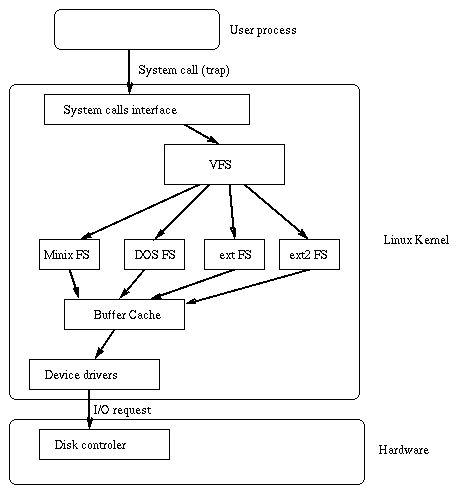
\includegraphics[width=0.65\textwidth]{ext2-vfs.png}
			\end{center}

		\end{enumerate}

\end{enumerate}

\subsection*{Módulos del kernel}

\begin{enumerate}
	\item \textbf{Módulo hello.c}

	Se compiló el módulo hello.c provisto en el enunciado utilizando el comando \textbf{make} con el \textit{Makefile} correspondiente (también provisto). Luego, con los comandos insmod y rmmod, se insertó y se quitó el módulo del kernel (respectivamente), mostrando en pantalla los mensajes indicados.

	\item \textbf{Un móludo propio: leds.c}

	A continuación, se muestra el código del módulo del kernel que termite controlar los LEDs del teclado tal como pide el enunciado:

	\begin{verbatim}
#include <linux/module.h>
#include <linux/init.h>
#include <linux/kernel.h> /* KERNEL_INFO, KERNEL_ALERT */
#include <linux/kd.h>		/* For KDSETLED */
#include <linux/vt.h>
#include <linux/vt_kern.h> /* For fg_console */
#include <linux/console_struct.h>	/* For vc_cons */

#include <linux/proc_fs.h> /* For proc */
#include <linux/string.h>
#include <linux/vmalloc.h> /* For vmalloc, vfree */
#include <asm/uaccess.h> /* For copy_from_user */

#define LED_ALLOFF  0x00
#define LED_SCROLL  0x01
#define LED_NUMLOCK  0x02
#define LED_CAPSLOCK  0x04

MODULE_LICENSE("GPL");

//TTY driver
struct tty_driver *leds_driver;
//Estructura de proc
static struct proc_dir_entry *proc_entry;
static char *input_leds;

ssize_t control_leds(struct file *filp, const char __user *buff, 
    unsigned long len, void *data) {

    int leds_code = LED_ALLOFF;
    
    //Copiamos la información leída del espacio de usuario
    //al espacio de memoria del kernel
    copy_from_user(&input_leds[0], buff, len);
    
    if(input_leds[0] == '1') {
        leds_code += LED_NUMLOCK;
    }
    if(input_leds[2] == '1') {
        leds_code += LED_CAPSLOCK;
    }
    if(input_leds[4] == '1') {
        leds_code += LED_SCROLL;
    }
    
    //Seteamos los leds via ioctl con KDSETLED
    (leds_driver->ioctl) (vc_cons[fg_console].d->vc_tty, NULL, KDSETLED, leds_code);
    
    printk(KERN_INFO "leds: Se han cambiado el estado de los LEDs\n");
    
    return len;
}

int iniciar_modulo(void) {

    //Pedimos memoria en espacio de kernel
    input_leds = (char *)vmalloc(PAGE_SIZE);
    
    if (!input_leds) {
        printk(KERN_ALERT "leds: No se pudo pedir memoria\n");
        return 1;
    } else {
        memset(input_leds, 0, PAGE_SIZE);

        //Creamos la entrada /proc/leds
        proc_entry = create_proc_entry("leds", 0644, NULL);

        if(proc_entry == NULL) {
            vfree(input_leds);
            printk(KERN_INFO "leds: No se pudo crear la entrada en /proc\n");
        } else {
            //Funcion al escribir en proc
            proc_entry->write_proc = control_leds; 
            proc_entry->owner = THIS_MODULE;
        }

        //Driver relativo a la consola actual
        leds_driver = vc_cons[fg_console].d->vc_tty->driver;
        
        printk(KERN_INFO "leds: El modulo ha sido cargado.\n");
    
        return 0;
    }
    
}

void detener_modulo(void) {
    //Eliminamos /proc/leds
    remove_proc_entry("leds", &proc_root);
    //Liberamos memoria pedida
    vfree(input_leds);

    printk(KERN_INFO "leds: Modulo ha sido descargado.\n");
}

module_init(iniciar_modulo);
module_exit(detener_modulo);
	\end{verbatim}

	Para hacer uso de este módulo, basta con enviar un \textit{string} 's'  a \textit{/proc/leds} indicando que LEDs se desean activar con el siguiente comando \textbf{echo \textit{s} $>$ /proc/leds}, donde s es el string en cuestión. Este último deberá estar compuesto por 3 números (que pueden ser $0$ o $1$) separados por espacios que indicarán el nuevo estado de los LEDs, donde el primero número se corresponde con el LED de NUM LOCK, el segundo con el de CAPS LOCK y el último con el de SCROLL LOCK. Por ejemplo, para activar NUM LOCK y SCROLL LOCK, el comando en cuestión será \textbf{echo ``1 0 1'' $>$ /proc/leds}.

\end{enumerate}

\section*{Temas del Sistema Operativo}

\begin{enumerate}
  \item \textbf{Comunicaci\'on}

    Para realizar transferencia de archivos entre la m\'aquina virtual y el sistema operativo anfitri\'on se opt\'o por utilizar carpetas compartidas. Esto se logr\'o mediante los siguientes pasos:
    \begin{itemize}
      \item Dentro de la m\'aquina virtual se accede a \textit{Directorios compartidos} dentro del men\'u \textit{Dispositivos}.
      \item Se selecciona la carpeta que se desea compartir en la m\'aquina anfitrion y se le asigna un nombre.
      \item Se ejecuta el comando \textbf{mount -t vboxsf 'nombre-carpeta' $/$mnt$/$} para montar la carpeta compartida en la m\'aquina virtual.
    \end{itemize}

  \item \textbf{File System}

    Los \textit{hardlinks} apuntan a una estructura llamada i-nodo que contiene información sobre el archivo al que hace referencia el link y punteros a los bloques de memoria física en donde está alojado dicho archivo. Cada i-nodo almacena en uno de sus campos la cantidad de links que existen al archivo al que referencia. De este modo, sólo se elimina un i-nodo, y su correspondiente archivo, cuando la cantidad de links al archivo es 0, es decir, si se elimina un \textit{hardlink}, pero siguen existiendo links al archivo, este no será eliminado.
    Un i-nodo contiene la siguiente información:
    \begin{itemize}
      \item Modo (tipo de archivo y permisos)
      \item Cantidad de links
      \item UID del owner
      \item GID del owner
      \item Tamaño del archivo (en bytes)
      \item Fecha en la que el archivo fue accedido por última vez
      \item Fecha en la que el archivo fue modificado por última vez
      \item Fecha en la que el i-nodo fue modificado por última vez
      \item 12 punteros a bloques
      \item 1 puntero indirecto a bloques
      \item 1 puntero doble indirecto a bloques
      \item 1 puntero triple indirecto a bloques
      \item Estado del i-nodo (flags)
      \item Cantidad de bloques que ocupa el archivo
      \item Campos extra o reservados
    \end{itemize}

  \item \textbf{Prioridades}

    Para lograr ejecutar procesos con distintas prioridades utilizamos el comando \textbf{nice}. En este caso se quieren ejecutar tres procesos (\textit{loop1}, \textit{loop2} y \textit{loop3}) y darle mayor prioridad a uno de ellos. Con este objetivo se ejecutaron los procesos \textit{loop1} y \textit{loop2} asignandoles una muy baja prioridad (\textbf{nice -15 ./loop1} y \textbf{nice -15 ./loop2}). Luego se ejecut\'o el proceso \textit{loop3} normalmente logrando asi que tenga m\'as prioridad que los otros procesos mencionados.

    Para verificar el uso del CPU por parte de cada uno de los procesos se utiliz\'o el comando \textbf{top}. De esta manera se obtuvieron los siguientes resultados:
    \begin{itemize}
      \item \textit{loop1}: 3.3\%
      \item \textit{loop2}: 3.3\%
      \item \textit{loop3}: 93.1\%
    \end{itemize}

  \item \textbf{Parámetros del Kernel}

	Una vez arrancado el sistema, el uso de la memoria RAM, sin considerar los \textit{caches/buffers}, es de tan sólo $14740$ KB. Para obtener esta información se utilizó el comando \textit{free} provisto por el sistema. 

	Una manera de reducir la cantidad de memoria utilizada consiste en detener procesos que se ejecuten en \textit{background} (llamados demonios) que no se estén utilizando. Por ejemplo, en este caso se pueden detener los demonios \textit{vboxadd-sevice}, \textit{vboxadd}, \textit{gmp} y \textit{cron} mediante el comando \textbf{sudo /etc/init.d/\textit{demonio} stop}. Al realizar esta operación, la memoria residente se redujo a $14450$ KB (información obtenida nuevamente con el comando \textbf{free}). Como se puede observar, la diferencia de uso es la memoria es muy pequeña. Esto se debe a que se trata de una distribución de Linux mínima que de por sí utiliza muy pocos recursos, por lo cual resulta prácticamente imposible reducir más su uso porque la gran mayoría de la memoria ocupada es utilizada por partes básicas y críticas del sistema operativo.

  \item \textbf{Swap}

	La cantidad de \textit{swap} disponible para el sistema es de $88316$ KB. Para determinar este valor se utilizó el mismo comando \textbf{free} utilizado en el punto anterior.

	Los sistemas basados en Linux, cuentan con la posibilidad de añadir más memoria \textit{swap} utilizando un archivo alojado en el disco rígido. Para realizar esta operación, en primer lugar se creó un archivo vacío de $10$ MB con el comando \textbf{sudo dd if=/dev/zero of=/mnt/10mb.swap bs=1M count=10}. Luego se le dió el formato adecuado con el comando \textbf{sudo mkswap /mnt/10mb.swap}. Finalmente, mediante el comando \textbf{swapon} se utilizó el archivo creado para expandir la cantidad de memoria \textit{swap} disponible del siguiente modo: \textbf{sudo swapon /mnt/10mb.swap}. Realizada esta operación, mediante el comando \textbf{free}, podemos ver que la cantidad de memoria \textit{swap} aumentó a $98356$ KB, unos $10$ MB tal como se esperaba.

	Para lograr que este cambio sea permanente basta con agregar la siguiente linea al archivo \textit{/etc/fstab}: 
	\begin{verbatim}
	/mnt/10mb.swap  none  swap  sw  0 0
	\end{verbatim}
	De este modo, al montarse los sistemas de archivos al inicio del sistema, se montará también nuestro archivo swap logrando así lo pedido.
 
\end{enumerate}

\section*{Promoción}

\begin{itemize}
	\item \textbf{Módulo \textit{mkdir}}

	Antes de mostrar el código del módulo en cuestión, vale hacer algunas aclaraciones. A partir de las últimas versiones del kernel de Linux, se hicieron distintos cambios para poder evitar que se pueda acceder a la tabla de \textit{System Calls} y para evitar que se pueda modificar la misma. Como primer medida básica de protección, la posición de dicha tabla no se encuentra disponible. Para poder obtener la dirección de dicha tabla, fue necesario recorrer la tabla de símbolos del kernel ubicada en el archivo de nombre \textit{System.map} y buscar la posición de memoria de la misma. Para esto, se utilizó el siguiente comando:

\begin{verbatim}
grep ' sys_call_table' /usr/src/linux/System.map |
sed “s/^\(.*\) \(.* sys_call_table\)/0x\1/”
\end{verbatim}

	Además de este inconveniente, el otro desafío consistia en poder modificar dicha tabla. El problema con esto, es que la zona de memoria donde se encuentra la misma es de sólo lectura, por lo cual fue necesario recurrir a funciones del kernel para poder marcar la página donde se encuentra dicha dirección de memoria como de lectura-escritura. A continuación, se muestra el código del módulo en cuestión donde se pueden observar en concreto las funciones utilizadas:

\begin{verbatim}
#include <linux/module.h>
#include <linux/kernel.h>
#include <linux/unistd.h>
#include <linux/mm.h>
#include <asm/cacheflush.h>

//Dirección de la sys_call_table
#define SYS_CALL_TABLE_ADDRESS 0xc0318500

MODULE_LICENSE ("GPL");

struct page *pg;
pgprot_t prot;

void **sys_call_table = (void *)SYS_CALL_TABLE_ADDRESS;

asmlinkage int (*original_sys_call) (const char *pathname);

//Función dummy para mkdir
asmlinkage int fake_mkdir_function(const char __user *pathname) {
    printk(KERN_ALERT "No se permite la ejecucion de mkdir!\n");

    return 0;
}

static int my_init (void) {
    //Guardo la llamada original a mkdir
    original_sys_call = sys_call_table[__NR_mkdir];

    //Marco la pagina asociada con permisos r-w-x
    pg = virt_to_page( SYS_CALL_TABLE_ADDRESS );
    prot.pgprot = VM_READ | VM_WRITE | VM_EXEC;
    change_page_attr(pg, 1, prot);
    
    //Modifico la entrada para asignarle la función dummy
    sys_call_table[__NR_mkdir] = fake_mkdir_function;

    return 0;
}

static void my_exit (void) {
    //Reestablezco la llamada original de mkdir
    sys_call_table[__NR_mkdir] = original_sys_call;
}

module_init(my_init);
module_exit(my_exit);
\end{verbatim}

	\item \textbf{Módulo \textit{/dev/probabilidad}}

	A continuación, se muestra el código del módulo que realiza las acciones pedidas:

\begin{verbatim}
#include <linux/kernel.h>
#include <linux/fs.h>
#include <linux/init.h>
#include <linux/miscdevice.h>
#include <linux/module.h>
#include <linux/vmalloc.h>
#include <linux/time.h>
#include <linux/proc_fs.h> /* For proc */
#include <asm/uaccess.h>

MODULE_LICENSE("GPL");

int acum_lecturas = 0;

static struct proc_dir_entry *proc_entry;

unsigned long prev_random;

static char *input_semilla;

//Funcion random
unsigned long get_random(unsigned long m_w, unsigned long m_z) {
    m_z = 36969 * (m_z & 65535) + (m_z >> 16);
    m_w = 18000 * (m_w & 65535) + (m_w >> 16);
    return (m_z << 16) + m_w;
}

//Funcion que retorna la cantidad de lecturas hasta el momento
int cant_lecturas( char *page, char **start, off_t off, 
    int count, int *eof, void *data ) 
{
    int len;
    len = sprintf(page, "Lecturas realizadas: %d\n", acum_lecturas);
    return len;
}

//Funcion para cambiar la semilla (escritura en proc)
ssize_t cambiar_semilla(struct file *filp, const char __user *buff, 
    unsigned long len, void *data) 
{

    copy_from_user(&input_semilla[0], buff, len);

    prev_random = simple_strtoul(input_semilla, NULL, 10);
    
    printk(KERN_INFO "probabilidad: Se han cambiado la semilla\n");
    
    return len;
}

//Funcion de lectura del dispositivo que retorna la letra aleatoria
static ssize_t probabilidad_read(struct file * file, char * buf, 
    size_t count, loff_t *ppos) 
{

    unsigned int random_pos;
    char *probabilidad_str;
    char random_letter;
    int len;

    //Para generar el numero aleatorio utilizo como semilla 
    //el numero anterior
    prev_random = get_random(prev_random, prev_random);

    //Obtengo una posicion aleatoria entre 1 y 25 
    //para obtener la letra del abecedario
    random_pos = (prev_random % 25);
    probabilidad_str = "ABCDEFGHIJKLMNOPQRSTUVWXYZ";
    random_letter = probabilidad_str[random_pos];
    len = 1;

    //Solo se puede leer el dispositivo en forma completa
    if (count < len)
        return -EINVAL;

    if (*ppos != 0)
        return 0;

    //Copio al buffer de espacio de usuario la letra aleatoria
    if (copy_to_user(buf, &random_letter, len))
        return -EINVAL;

    *ppos = len;

    //Registro una nueva lectura al dispositivo
    acum_lecturas++;

    printk(KERN_ALERT "probabilidad: Se ha utilizado la semilla 
       %lu\n", simple_strtoul(input_semilla, NULL, 10));

    return len;
}

//Operaciones del dispositivo
static const struct file_operations probabilidad_fops = {
    .owner = THIS_MODULE,
    .read = probabilidad_read, //Funcion de lectura de proc
};

//Estructura del dispositivo
static struct miscdevice probabilidad_dev = {
    MISC_DYNAMIC_MINOR,
    "probabilidad",
    &probabilidad_fops
};

static int __init probabilidad_init(void) {
    int ret;

    //Crea el dispositivo 'probabilidad' de tipo misc
    ret = misc_register(&probabilidad_dev);
    if (ret) {
        printk(KERN_ERR "No se puede registrar el 
          dispositivo 'probabilidad'\n");
    } else {

        //Utilizo la hora actual (en ns) como semilla inicial
        //al cargar el módulo
        struct timespec tv;
        getnstimeofday(&tv);
        prev_random = tv.tv_nsec;
        
        input_semilla = (char *)vmalloc(PAGE_SIZE);
        memset(input_semilla, 0, PAGE_SIZE);

        proc_entry = create_proc_entry("probabilidad", 0644, NULL);
    
        if(proc_entry == NULL) {
            printk(KERN_INFO "probabilidad: No se pudo crear la 
              entrada en /proc\n");
        } else {
            proc_entry->read_proc = cant_lecturas;
            proc_entry->write_proc = cambiar_semilla;
            proc_entry->owner = THIS_MODULE;
        }
    }

    return ret;
}

static void __exit probabilidad_exit(void) {
    //Elimino la entrada de proc
    remove_proc_entry("probabilidad", &proc_root);
    vfree(input_semilla);
    //Elimino el dispositivo
    misc_deregister(&probabilidad_dev);
}

module_init(probabilidad_init);
module_exit(probabilidad_exit);
\end{verbatim}  

	El presente módulo se encarga de crear un dipositivo de tipo MISC en /dev/probabilidad que, al ser leído, retorna una letra aleatoria. Para leer el dispositivo, basta con ejecutar el comando \textbf{cat /dev/probabilidad}. Además, provee la opción de cambiar la semilla utilizada para ir generando la secuencia aleatoria, mediante el comando \textbf{echo \textit{semilla} /proc/probabilidad}. Por otro lado, tal como pide el ejercicio, este módulo permite retornar la cantidad de veces que fue leído.

	\item \textbf{Scheduling y Administración de memoria en Windows}

	\begin{itemize}
		\item \textbf{Scheduling}

		Windows utiliza un esquema de \textit{scheduling} basado en prioridades. A cada proceso se le asigna una prioridad, que puede ir desde 0 (prioridad más baja) hasta 31 (prioridad más alta). Sin embargo, sólo el proceso zero-page, encargado de asignar ceros a las páginas libres cuando ningún otro proceso se está ejecutando, es el único que puede tener prioridad 0.

		El \textit{scheduler} trata de la misma manera a todos los procesos con igual prioridad. Es decir, utiliza un modelo de \textit{round-robin} para procesos con la misma prioridad. El scheduler chequea si existe algún proceso listo para ejecutar en el nivel de prioridad más alto. Si no llega a encontrar ningún proceso en ese nivel, pasa a buscar en el siguiente nivel de prioridad. En el caso de que un proceso de mayor prioridad pase a estar listo durante la ejecución de un proceso de menor prioridad, el scheduler interrumpirá la ejecución de este último para poder ejecutar el proceso de mayor prioridad.
		Para determinar la prioridad de cada uno de los procesos, el scheduler se vale de dos estructuras llamadas clase de prioridad y nivel de prioridad.

		\item \textbf{Administración de memoria}

		En los sistemas Windows el espacio de memoria virtual está dividido en 2 secciones: espacio de usuario y espacio de sistema. En arquitecturas de 32 bit, los 2 GB de memoria virtual más bajos están asignados al usuario, mientras que los 2 GB de direcciones más altas, al sistema. Sin embargo, la memoria asignada al usuario se puede extender hasta 3 GB.
		
		En cuanto al manejo de memoria, los sistemas Windows utilizan paginación por demanda. Para poder mapear direcciones virtuales a direcciones físicas Windows utiliza dos páginas de tablas. Cada página de memoria virtual tiene una entrada en la página de tablas. A partir de la información que se encuentra en cada entrada de la tabla de páginas se puede conocer la página física a la que referencia dicha página virtual. En máquinas de 32 bits, se utilizan dos niveles de tablas, es decir, una es un índice a un directorio de páginas y la segunda apunta directamente a la página de memoria física. El esquema de mapeo de memoria virtual a memoria física se puede representar con el siguiente esquema.

		\begin{center}
		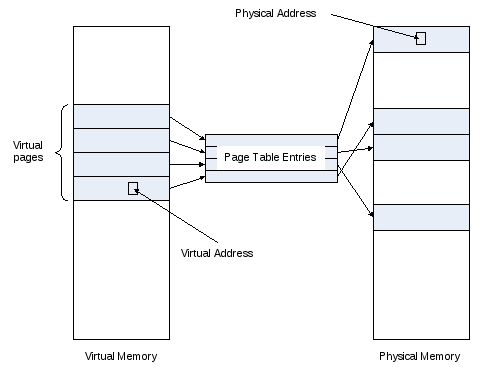
\includegraphics[width=0.7\textwidth]{virtual.png}
		% virtual.png: 0x0 pixel, 300dpi, 0.00x0.00 cm, bb=
		\end{center}
	\end{itemize}

\end{itemize}

\section*{Referencias}
\begin{itemize}
 	\item Hijacking Linux Syscalls \& Writing a Linux Keylogger: A Case Study 

	(www.epanastasi.com/?page\_id=52)
	\item sys\_call\_table module 

	(blinkeye.ch/dokuwiki/doku.php/projects/lkm)
	\item Access the Linux kernel using the /proc filesystem 

	(www.ibm.com/developerworks/linux/library/l-proc.html)
	\item Console IOCTLs Under Linux 

	(www.w00w00.org/files/articles/conioctls.txt)
	\item 	The Linux Kernel Module Programming Guide: Chapter 7. Talking To Device Files

			The Linux Kernel Module Programming Guide: Chapter 10. Replacing Printks

			(www.linuxtopia.org/online\_books/Linux\_Kernel\_Module\_Programming\_Guide/)

	\item Scheduling Priorities - Windows 

			(http://msdn.microsoft.com/en-us/library/ms685100(VS.85).aspx)

\end{itemize}


\end{document}